\documentclass[10pt]{llncs}

\sloppy
\usepackage{amsfonts}

\usepackage{algorithm}
\usepackage{algorithmic}
\usepackage{graphicx}
\usepackage{wrapfig}
\graphicspath{{Figures/}}

\newcommand{\exist}{{\sc Exist}}
\newcommand{\GBWT}{\mathit{GBWT}}
\newcommand{\B}{\mathit{B}}

\usepackage{tikz}
\usetikzlibrary{arrows,backgrounds}

\makeindex
\begin{document}

\title{Computing Lempel-Ziv Factorization Online}

\institute{Lomonosov Moscow State University, Moscow, Russia\\ tat.starikovskaya@gmail.com}

\author
{
   Tatiana Starikovskaya
}
\date{\empty}
\maketitle

\begin{abstract}
We present an algorithm which computes the Lempel-Ziv factorization of a word  of length  on an alphabet  of size  online in the following sense: it reads  starting from the left, and, after reading each  characters of , updates the Lempel-Ziv factorization. The algorithm requires  bits of space and  time. The basis of the algorithm is a sparse suffix tree combined with wavelet trees.
\end{abstract}

\section{Introduction}
The Lempel-Ziv factorization (further LZ-factorization for short) of a word  is a decomposition , where a factor , , is either a character that does not occur in  or the longest prefix of  that occurs in  at least twice~\cite{Crochemore:1986:TR:21537.21539,Ziv77auniversal}.

The most famous application of the LZ-factorization is data compression (e.g. the LZ-factorization is used in gzip, WinZip, and PKZIP). Moreover, it is a basis of several algorithms~\cite{Kolpakov99findingmaximal,Gusfield:2004:LTA:1046081.1046083} and text indexes~\cite{Kreft:2011:SBL:2018243.2018251}.

Let  be a word of length  on an alphabet  of size . There are many algorithms that compute the LZ-factorization in  bits of space~\footnote{In this paper  stands for .}. These algorithms use suffix trees~\cite{Rodeh:1981:LAD:322234.322237}, suffix automata~\cite{Crochemore:1986:TR:21537.21539} or suffix arrays~\cite{Abouelhoda:2004:RST:985384.985389,journals/mics/ChenPS08,Crochemore:2008:CLP:1346353.1346507,conf/iwoca/CrochemoreIIKRW09,Crochemore:2008:SAC:1395764.1395899,Ohlebusch:2011:LFR:2018243.2018249} as a basis.

However, only two algorithms have been known which use  bits of space~\cite{Okanohara:2008:OAF:1431008.1431068,Ohlebusch:2011:LFR:2018243.2018249}. The algorithms exploit similar ideas (both are based on an FM-index and a compressed suffix array). The algorithm~\cite{Ohlebusch:2011:LFR:2018243.2018249} is offline and requires  time.

Running time of the algorithm~\cite{Okanohara:2008:OAF:1431008.1431068} is rather big, , but the algorithm computes the LZ-factorization of a word  online. Consider the factors  of the LZ-factorization of a word . The LZ-factorization of a word , where  is a character, contains either  or  factors: in the first case the factors are , where the last factor ; and in the second case the factors are , where . The algorithm reads  and after reading each new character updates the LZ-factorization, i.e. either increases the length of the last factor by one or adds a new factor.

For many practical applications dealing with large volumes of data it would be natural to allow updating the LZ-factorization only each  new characters of , for some small parameter , in order to reduce the running time. Unfortunately, naive application of this idea to the algorithm~\cite{Okanohara:2008:OAF:1431008.1431068} does not improve its running time.

Here we propose a new linear-space algorithm which achieves a reasonable trade-off between frequency of updates and running time. The algorithm updates the LZ-factorization of  each  characters of , requiring  time and  bits of space. It is assumed that both  and  are known beforehand and . The basis of the algorithm is a sparse suffix tree combined with wavelet trees.

Let  be a word of length  on . Throughout the paper, positions in  are numbered from~. The subword of  from position  to position  (inclusively) is denoted by . If , then we write  instead of . A word  is called a suffix of  and a word  is called a prefix of .

With each word  of length  on  we associate a meta-character  formed by concatenating bit representations of characters of . Note that a bit representation of any character of  can be obtained from the bit representation of  in constant time by two shift operations. Also,  can be obtained from  in  time.

\section{Algorithm}
Let  be the factors of the LZ-factorization of . For the sake of clarity we describe not how to update the LZ-factorization after reading each block of characters but rather how to compute  sequentially. However, it will be easy to see that the presented algorithm can be modified to solve the problem we formulated in the introduction.

Suppose that  of total length  have been computed. The algorithm consists of two procedures. The procedure  checks if  is less than  and, if it is, computes  (Section~\ref{sec:<r}). The procedure  computes  only if it is already known that  (Section~\ref{sec:>r}). To compute  the algorithm runs  first and then, if necessary, runs .

\subsection{Data Structures}
The algorithm makes use of several data structures. To explain what these data structures are, we need to give a definition of a trie and a compacted trie first.

\begin{definition}
A trie for a set of words  is a rooted tree edges of which are labelled by characters. For each prefix  of a word  there exists exactly one vertex such that  is spelled out by the path from the root of the trie to this vertex, and vice versa, a word spelled out by any path starting at the root must be a prefix of one of the words . A compacted trie for  can be constructed from the trie by eliminating all vertices with one son, thus forming edges that are labelled by words rather than single characters.
\end{definition}

The algorithm reads  by blocks of  characters starting from the left. After reading the -th block of , the first data structure is an (uncompacted) trie on suffixes of words , . Each explicit vertex  of the trie stores the leftmost starting position of a suffix ending in the subtree rooted at .

Let  be the meta-word formed by replacing each block of characters of  with the corresponding meta-character. The second data structure is an implicit suffix tree for , i.e. a compacted trie for the set of suffixes of . This tree is also called a sparse suffix tree for ~\cite{ChienHonShahVitterDCC08,HonShahThanVitterSPIRE09,ChiuHonShahVitterDCC10}, though the original definition of a sparse suffix tree is slightly different~\cite{KU-96}. 

For each explicit vertex  of the suffix tree we store a compacted trie  on words of length  corresponding to the first meta-characters on the edges outgoing from .

\begin{definition}
   Consider a tree with labels on edges (a suffix tree or a trie). We say that a word  is \emph{represented} by a vertex  (or that  \emph{represents} ), if the word spelled out by the path from the root of the tree to  is equal to .
\end{definition}

If the label of an edge  of the suffix tree begins with a meta-character , and  is the corresponding word of length , then we store a pointer to the edge  in the leaf of  representing . Tries in vertices are used for navigation in the suffix tree (but not only for it). Clearly, given a vertex  and a meta-character , it takes  time to find an edge  such that its label starts with .

Also, the algorithm maintains a dynamic data structure which allows, given a vertex  of the suffix tree, to compute the ranks of the leftmost and the rightmost leaves of the subtree rooted at  in  time. 

\begin{definition}
	Block borders are positions of  of the form , .
\end{definition}

Finally, we store a data structure which allows, given an interval , a word , and a block border , to determine whether a set of block borders corresponding to the starting positions of the suffixes which are represented by the leaves of the suffix tree with ranks in the interval  contains a block border different from  and preceded by an occurrence of . The procedure \exist returns zero if there is no such block border and one of them otherwise.

Details of implementation are not important to understand the algorithm and will be explained later, in Section~\ref{sec:DS}.

Hereafter  is denoted by . We assume that the algorithm has read the first  blocks of  before running the procedures  and .

\subsection{Procedure }
\label{sec:<r}
Let  be the longest prefix of  which occurs before the position . Obviously,  if  (see Fig.~\ref{fig:LM1}), and   if .

\begin{figure}[h!]
    \begin{center}
	  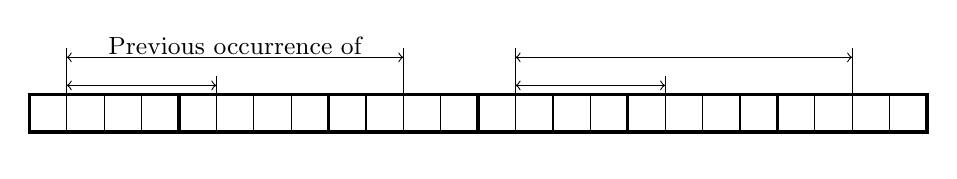
\begin{tikzpicture}[scale=0.95]
    \filldraw[very thick, fill=white] (0,0) rectangle (12,0.5);
    
    \foreach \x in {0.5,1,...,11.5} {
    	\draw (\x,0) -- (\x,0.5);
    }
    
    \foreach \x in {2,4,6,8,10} {
    	\draw[very thick] (\x,0) -- (\x,0.5);
    }
    
    \node[below] at (0.25,0) {\small{}};
    \node[below] at (3.75,0) {\small{}};
    \node[below] at (6.25,0) {\small{}};

    \draw (0.5,0) -- (0.5,1.125);
    \draw (5,0) -- (5,1.125);
    \draw (2.5,0) -- (2.5,0.75);
    
    \draw[<->] (0.5,1) -- (5,1)
    	node[pos=0.5,yshift=0.15cm]{\small{Previous occurrence of }};
    \draw[<->] (0.5,0.625) -- (2.5,0.625)
    	node[pos=0.5,yshift=0.15cm]{\tiny{}};

    \draw (6.5,0) -- (6.5,1.125);
    \draw (11,0) -- (11,1.125);
    \draw (8.5,0) -- (8.5,0.75);
    \draw[<->] (6.5,1) -- (11,1)
    	node[pos=0.5,yshift=0.15cm]{\small{}};
    \draw[<->] (6.5,0.625) -- (8.5,0.625)
    	node[pos=0.5,yshift=0.15cm]{\tiny{}};
\end{tikzpicture}       \caption{Case , . Block borders are in bold.}
      \label{fig:LM1}
    \end{center}
\end{figure}

 first computes the longest prefix  of  which occurs before the position . It traverses the trie starting at the root and following edges labelled by the characters of . The algorithm stops in a vertex  either when  has no outgoing edge labelled by the next character of  or when the position stored in the next vertex is bigger than  (which means that its label does not occur at positions ).

Clearly,  will be labelled by . If , then . Otherwise, the algorithm reads , updates the data structures and proceeds the traverse in a similar manner this time starting at  and following edges labelled by the characters of . A vertex  the procedure will stop at will be labelled by .

From the definition of a trie it follows that the traverse will take  time.

\subsection{Procedure }
\label{sec:>r}
 consists of two steps. The first can be considered as preliminary, and during the second step we compute . 

\subsubsection{The First Step}
 starts with reading . After reading the -th block, it updates the data structures and checks whether  is represented by a leaf of the suffix tree of . If it is,  proceeds to the second step. From the definition of a suffix tree it follows that after the first step of  all suffixes starting at positions less than  will be represented by leaves.

\begin{lemma}
\label{lm:prelim}
During the first step at most  characters of  will be read.
\end{lemma}
\begin{proof}
Since  is the minimal position such that  is represented by a leaf,  is represented by an inner vertex in the suffix tree of  and, consequently, occurs before the position  in . Therefore,  occurs before the position  (see Fig.~\ref{fig:LM2}) and . The statement of the lemma easily follows.
\end{proof}

\begin{figure}[h!]
    \begin{center}
      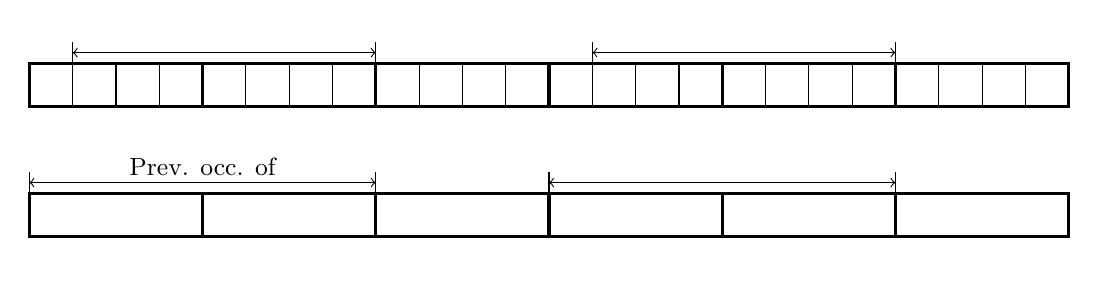
\begin{tikzpicture}[scale=1.1]
    \filldraw[very thick, fill=white] (0,0) rectangle (12,0.5);
    
    \foreach \x in {0.5,1,...,11.5} {
    	\draw (\x,0) -- (\x,0.5);
    }
    
    \foreach \x in {2,4,6,8,10} {
    	\draw[very thick] (\x,0) -- (\x,0.5);
    }
    
    \node[below] at (6.25,0) {\small{}};
	\node[below] at (11.75,0) {\small{}};

    \draw (0.5,0) -- (0.5,0.75);
    \draw (4,0) -- (4,0.75);
    \draw[<->] (0.5,0.625) -- (4,0.625)
    	node[pos=0.5,yshift=0.2cm]{\small{}};
    
    \draw (6.5,0) -- (6.5,0.75);
    \draw (10,0) -- (10,0.75);
    \draw[<->] (6.5,0.625) -- (10,0.625)
    	node[pos=0.5,yshift=0.2cm]{\small{}};
   
   
   \filldraw[very thick, fill=white] (0,-1.5) rectangle (12,-1);
             
   \foreach \x in {2,4,6,8,10} {
   	\draw[very thick] (\x,-1.5) -- (\x,-1);
   }
       
   \node[below] at (7,-1.5) {\small{}};
   \node[below] at (11,-1.5) {\small{}};
   
   \draw (0,-1.5) -- (0,-0.75);
   \draw (4,-1.5) -- (4,-0.75);
   \draw[<->] (0,-0.875) -- (4,-0.875)
   	node[pos=0.5,yshift=0.2cm]{\small{Prev. occ. of }};
       
   \draw (6,-1.5) -- (6,-0.75);
   \draw (10,-1.5) -- (10,-0.75);
   \draw[<->] (6,-0.875) -- (10,-0.875)
   	node[pos=0.5,yshift=0.2cm]{\small{}}; 
\end{tikzpicture}       \caption{Relation between  and .}
      \label{fig:LM2}
    \end{center}
\end{figure}

We initialize  with . From the proof of the lemma it follows that . During the computation process we will increase  until, finally, it will become equal to .

Furthermore, the lemma guarantees that after the first step the difference between the position of the last read character of  and  is less than . This invariant will be maintained throughout the second step of the procedure as well in the following way: we will read a new block of characters and update the data structures only when  is equal to the position of the last read character of .

\subsubsection{The Second Step}
Consider the first block border which intersects a previous occurrence of  (see Fig.~\ref{fig:LM3}). It divides the occurrence into two parts: the first short part equal to  and the second part equal to a prefix of , .

\begin{figure}[h!]
    \begin{center}
      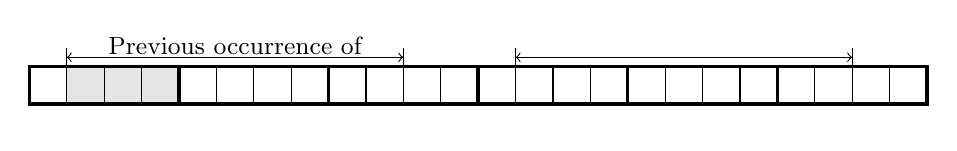
\begin{tikzpicture}[scale=0.95]
    \filldraw[very thick, fill=white] (0,0) rectangle (12,0.5);
    \filldraw[fill=gray!20] (0.5,0) rectangle (2,0.5);
    \draw[very thick] (0.5,0) -- (2,0);
    \draw[very thick] (0.5,0.5) -- (2,0.5);
    
    \foreach \x in {0.5,1,...,11.5} {
    	\draw (\x,0) -- (\x,0.5);
    }
    
    \foreach \x in {2,4,6,8,10} {
    	\draw[very thick] (\x,0) -- (\x,0.5);
    }
    
    \node[below] at (0.25,0) {\small{}};
    \node[below] at (3.75,0) {\small{}};
    \node[below] at (6.25,0) {\small{}};

    \draw (0.5,0) -- (0.5,0.75);
    \draw (5,0) -- (5,0.75);
    
    \draw[<->] (0.5,0.625) -- (5,0.625)
    	node[pos=0.5,yshift=0.15cm]{\small{Previous occurrence of }};

    \draw (6.5,0) -- (6.5,0.75);
    \draw (11,0) -- (11,0.75);
    \draw[<->] (6.5,0.625) -- (11,0.625)
    	node[pos=0.5,yshift=0.15cm]{\small{}};
\end{tikzpicture}       \caption{A previous occurrence of . The part equal to  () is highlighted in grey.}
      \label{fig:LM3}
    \end{center}
\end{figure}

Let  be the longest prefix of  with at least one occurrence at a block border which is less than  and preceded by an occurrence of . Obviously, . 

For each  the procedure  either computes  and updates  or proves that  and starts computation of .

If , then the second step of  starts with computing the length  of the longest common prefix of   and . In order to compute  the procedure compares the two strings character by character. If , the procedure puts  equal to . Then the procedure starts to work with the suffix tree.

The procedure traverses the suffix tree starting at the root and following the edges so that characters of the words corresponding to meta-characters of labels coincide with characters of . For navigation the procedure uses compact tries stored in the vertices of the suffix tree.

Suppose that after reading a word  of length at least  the procedure is on the edge  of the suffix tree. Two cases are possible depending on whether  is an inner vertex of the suffix tree or a leaf.

Let  be an inner vertex. Obviously,  iff a set of the block borders corresponding to the leaves of the subtree rooted at  contains a block border less than  preceded by an occurrence of .

\begin{definition}
  \emph{String depth} of a vertex  of the suffix tree is the length of its label.
\end{definition}

\begin{lemma}
\label{lm:B_v_prop}
 Let  be an explicit inner vertex of the suffix tree of  with string depth at least . Then a block border corresponding to a leaf in the subtree rooted at  can not be bigger than .
\end{lemma}
\begin{proof}
  Indeed, a subtree rooted at  can only contain leaves representing suffixes of length at least , and all such suffixes start at positions . The statement immediately follows.
\end{proof}

Since , the string depth of  is at least . It follows from the lemma that a set of the block borders corresponding to the leaves of the subtree rooted at  might contain only one block border situated to the left of , namely, . 

Let  and  be the ranks of the leftmost and the rightmost leaves of the subtree rooted at . The ranks  and  can be computed in  time (see Section~\ref{sec:DS}). Then the set of the block borders corresponding to the leaves of the subtree rooted at  contains a block border less than  preceded by an occurrence of  iff the set of block borders corresponding to leaves with ranks belonging to the interval  contains at least one block border different from  and preceded by an occurrence of . To define is this condition holds we call the procedure \exist{}. If such a block border exists, the procedure updates  and proceeds. Otherwise, the procedure starts computation of .

If  is a leaf then instead calling the procedure \exist{} we first check if this leaf corresponds to a block border less than  and then check if the border is preceded by an occurrence of  using a character-by-character comparison. 

Suppose now that after reading  of length at least  the procedure stops on an edge  of the compact trie , stored in a vertex  of the suffix tree (which means that we are looking for an edge outgoing from  which has an appropriate label). Let  and  be sons of , which correspond to the leftmost and the rightmost leaves of the subtree of  rooted at . Obviously,  and  can be found in  time. All block borders corresponding to leaves with ranks  are the starting positions of occurrences of . Moreover, if one of these block borders is bigger than  then it is equal to  (Lemma~\ref{lm:B_v_prop}). To define if there is a block border corresponding to a leaf with the rank in the interval  preceded by an occurrence of  and different from  the algorithm calls the procedure \exist{}.

Correctness of the procedure  follows from its description. The following lemma estimates the time spent during , not including the time for updates of the data structures.

\begin{lemma}
\label{lm:second_step}
To compute  the procedure  needs  time.
\end{lemma}
\begin{proof}
During the first step  reads  characters of  (Lemma~\ref{lm:prelim}).

To compute the longest common prefix of  and  we need  time. To follow  down in the suffix tree we need  time. Since after each execution of the procedure \exist{} we either increase  or proceed to the computation of , it is executed at most  times. The procedure \exist{} takes  time (see Section~\ref{sec:DS}). Therefore, the total time spent during the second step of  is .
\end{proof}


\section{Data Structures}
\label{sec:DS}
As we have already said, our algorithm maintains two data structures. In this section we give the details and describe update procedures.

\subsection{Trie}
After reading  the trie contains suffixes of words , . To update the trie after reading the -th block of characters we first check if  is represented in the trie. To do that we traverse the trie starting at the root and following edges labelled by the characters of . If we read out the whole word, then , and, consequently, all its suffixes are represented in the trie. If not, we add all suffixes of , including the word itself, to the trie. 

\begin{lemma}
\label{lm:CT}
The trie occupies  bits of space and its maintenance takes  time.
\end{lemma}
\begin{proof}
Due to our choice of , there are at most  different words of length  on . Therefore, the trie has at most  vertices and occupies  bits of space.

To check if the words , , are represented in the trie one needs  time in total. During the algorithm we add suffixes of at most  words. All suffixes of a word of length  can be added to the trie in  time, so we get the announced time bound.
\end{proof}

Finally, suppose that we create a new vertex  in the process of adding a suffix  of the word  to the trie. Then we just remember the position  as the leftmost starting position of a suffix ending in the subtree rooted at . This completes the description of the update procedure of the trie.

\subsection{Suffix Tree}
The suffix tree is updated by Ukkonen's algorithm~\cite{ukkonen:on-line}. When we create a new edge outgoing from a vertex  with the first character of the label equal to , we add  to .

Below we describe the procedure \exist{} and how to compute the ranks of the leftmost and the rightmost leaves in a subtree rooted at a vertex .

\subsubsection{Ranks of the leftmost and the rightmost leaves}
The data structure we will use to compute the ranks of the leftmost and the rightmost leaves of a subtree is similar to the one from~\cite{KNS12}.

We maintain a dynamic doubly-linked list  corresponding to the Euler tour of the current suffix tree. Each internal vertex of the suffix tree is stored in two copies in , corresponding respectively to the first and last visits of the vertex during the Euler tour. Leaves of the suffix tree are kept in one copy. Observe that the leaves of the suffix tree appear in  in the ``left-to-right'' order, although not consecutively.

We also maintain a balanced binary tree, denoted , whose leaves are elements of . Note that the number of vertices of  is bounded by  and the height of~ is . We call leaves of  corresponding to leaves of the suffix tree {\em suffix leaves}. For each suffix leaf we store the corresponding block border (we will use this information in the procedure \exist{}), and for each internal vertex  of~ we store the number of suffix leaves in the subtree of~ rooted at~.

The rank of the leftmost leaf in the subtree rooted at  is the number of the suffix leaves in  preceding the first copy of  in  plus one. This number can be computed in  time by following the path from the leaf of  corresponding to this copy to the root of  and summing up the number of the suffix leaves in the subtrees rooted at the left sons of the vertices on the path. The rank of the rightmost leaf can be computed in a similar way.

Now we should explain how to update  and . When a new vertex  is added to a suffix tree, the following updates should be done (in order):

\begin{itemize}
\item[(i)] insert  at the right place of the list  (in two copies if  is an internal vertex),
\item[(ii)] rebalance the tree  if needed,
\item[(iii)] if  is a leaf of the suffix tree (i.e. a suffix leaf of ), update information about the number of suffix leaves in .
\end{itemize}

To see how update (i) works, we have to recall how suffix tree is updated when a new document is inserted. Two possible updates are creation of a new internal vertex  by splitting an edge into two (edge subdivision) and creating a new leaf  as a child of an existing vertex. In the first case, we insert the first copy of  right after the first copy of its parent, and the second copy right before the second copy of its parent. In the second case, the parent of  has already at least one child, and we insert  either right after the second (or the only) copy of its left sibling, or right before the first (or the only) copy of its right sibling. 

Rebalancing the tree  (update (ii)) is done using standard methods. Observe that during the rebalancing we may have to adjust the information about the number of the suffix leaves for internal vertices, but this is easy to do as only a constant number of local modifications is done at each level.

Update (iii) is triggered when a new leaf  is created in the suffix tree and added to . We then have to follow the path in  from the new leaf  to the root and update the information about the number of suffix leaves for all vertices on this path. These updates are
straightforward. All these steps take  time. 

\subsubsection{Procedure \exist}
Let  be the starting position of the suffix represented by the -th leaf in the left-to-right order on the leaves of the suffix tree. Consider a virtual sequence , where  is equal to the reverse of the bit representation of . Elements of  belong to a segment .

Consider a dynamic wavelet tree for . The wavelet tree for a sequence , elements of which belong to a segment  can be defined recursively. If  then the wavelet tree consists of one vertex corresponding to . Otherwise the tree has a root corresponding to the segment . A binary vector  is defined as follows: if , then , otherwise . We store a data structure~\cite{Makinen:2008:DES:1367064.1367072} which allows ro read any bit , compute the number of zeros or ones in a prefix  ( or  ), or compute the position of -th zero or -th one ( or ), as well as to add a new bit between  and  in  time. The data structure occupies the number of bits proportional to the vector's length. Let  be a subsequence of  formed by the elements , , and  be the complementary subsequence. Then a subtree rooted at the left son of the root is the wavelet tree for , elements of which belong to a segment , and a subtree rooted at the right son of the root is the wavelet tree for , elements of which belong to a segment .

It follows from the definition that the wavelet tree for  has  leaves and, consequently,  vertices. As there are at most  levels in the tree and the total length of the bit vectors is at most , the wavelet tree for  occupies  bits of space in total.

We define a meta-character  as follows: reverse the bit representation of  and then append  zeros to it. A meta-character  is defined in a similar way, but ones are appended instead of zeros. Obviously, a block border  is preceded by an occurrence of  iff the reverse of the bit representation of  lies in the interval . Let  be the set of block borders corresponding to the leaves with ranks in  and preceded by an occurrence of . First the procedure \exist{} finds  such that , and then computes the block borders  corresponding to leaves with ranks . Obviously,  contains at least one block border different from  iff either  or  is not equal to .

The dynamic wavelet tree for  allows to find  such that  belong to  in  time~\cite{Makinen06position-restrictedsubstring}. We start at the interval  of . Now we map the interval to the left and to the right, replacing  by  and  by , and continue recursively. We stop the recursion (i) if the interval  is empty; (ii) if the interval corresponding to the current vertex does not intersect with the interval ; (iii) if the interval corresponding to the current vertex is contained in . It can be shown that only  vertices will be visited. Suppose that the traverse stops at some vertex  because of (iii) and  is the corresponding subsequence of . Then elements  belong to the interval , and their positions in  belong to . Any of these positions, e.g., the position of an element  in , can be computed in  time in the following way: we go along the path from  to the root replacing  by  when moving from the left (right) son of a vertex  to . The value of  at the root will be equal to the position of the element  in .

Using  the block borders corresponding to the leaves of the suffix tree with ranks  and  can be computed in  time, since it is enough to find the corresponding suffix leaves of~. Hence,  time is sufficient to determine whether a set of block borders corresponding to the starting positions of the suffixes which are represented by the leaves of the suffix tree with ranks in the interval  contains a block border different from  and preceded by an occurrence of .

It remains to describe how the wavelet tree is updated. To add a new element between  and  we need  time, because we need to create at most  vertices and to add a new bit to  binary vectors. To update the wavelet tree after adding a new leaf to the suffix tree we first compute the rank of this leaf in the left-to-right order on the leaves of the suffix tree in  time using  and then add the corresponding element to .

\begin{lemma}
\label{lm:ST}
The suffix tree and additional data structures occupy  bits and their maintenance takes  time.
\end{lemma}
\begin{proof}
The suffix tree has at most  leaves and therefore  edges. We specify labels of edges by their starting and final positions in . Hence, the suffix tree occupies  bits.

Tries in vertices of the suffix tree have  leaves in total and occupy  bits as well (labels of edges are specified by their starting and final positions in ). Finally, ,  and the dynamic wavelet tree use  bits of space.

Ukkonen's algorithm~\cite{ukkonen:on-line} takes  time (additional  appears because of the cost of navigation). To update tries in the vertices of the suffix tree we need  time. All wavelet tree updates take  time. And finally, updates of  and  take  time.
\end{proof}

\section{Results and Conclusions}
To conclude, we prove the following theorem. 

\begin{theorem}
  The presented algorithm computes the Lempel-Ziv factorization of a word  in  time and  bits of space.
\end{theorem}
\begin{proof}
Lemmas~\ref{lm:CT} and~\ref{lm:ST} guarantee that the data structures occupy  bits of space in total and that their maintenance takes  time.

To compute , first  is run. As we have proved, it takes  time.  is run only when  (i.e., at most  times) and takes  time. Therefore, the total time spent by procedures  and  is , and this completes the proof.
\end{proof}

It is easy to see that the described algorithm can be implemented online with the same running time and space.

\paragraph{Acknowledgement} 
The author has been supported by a grant 10-01-93109-CNRS-a of the Russian Foundation for Basic Research and by the mobility grant funded by the French Ministry of Foreign Affairs through the EGIDE agency.

The author thanks Simon J. Puglisi, who proposed to consider the problem of computation of the Lempel-Ziv factorization on a sparse suffix tree, and Gregory Kucherov and Alexei Lvovich Semenov for very helpful discussions.

\bibliographystyle{plain}
\bibliography{main}

\end{document}